%====================================================================
% ThreatLens: LLM-Agentic Compliance and Threat Modeling Engine
% IEEE Conference Proceedings format (IEEEtran, conference mode)
% Build: pdflatex -> pdflatex   (bibliography is inline; no BibTeX needed)
%====================================================================
\documentclass[conference]{IEEEtran}
\IEEEoverridecommandlockouts
% The preceding line is only needed to identify funding in the first footnote.
% If that is unneeded, please comment it out.
\usepackage{cite}
\usepackage{amsmath,amssymb,amsfonts}
\usepackage{algorithmic}
\usepackage{graphicx}
\usepackage{textcomp}
\usepackage{xcolor}
\usepackage[T1]{fontenc}
\usepackage[utf8]{inputenc}
\usepackage{booktabs}
\usepackage{array}
\usepackage{tabularx}
\usepackage{enumitem}
\usepackage{listings}
\usepackage{tikz}
\usetikzlibrary{arrows.meta,positioning}
\usepackage{microtype}
\usepackage{flushend}   % balances columns on the last page
\usepackage[hidelinks]{hyperref}
\usepackage{cleveref}   % must be loaded after hyperref

\def\BibTeX{{\rm B\kern-.05em{\sc i\kern-.025em b}\kern-.08em
    T\kern-.1667em\lower.7ex\hbox{E}\kern-.125emX}}

\hypersetup{pdftitle={ThreatLens: An LLM-Agentic Compliance and Threat Modeling Engine},
            pdfauthor={Jignesh}}

% ── Cross-reference names (IEEE style: "Fig. 1", "Table I", "Section II")
\crefname{figure}{Fig.}{Figs.}
\Crefname{figure}{Fig.}{Figs.}
\crefname{table}{Table}{Tables}
\Crefname{table}{Table}{Tables}
\crefname{section}{Section}{Sections}
\Crefname{section}{Section}{Sections}
\crefname{lstlisting}{Listing}{Listings}
\Crefname{lstlisting}{Listing}{Listings}
\renewcommand{\lstlistingname}{Listing}

% ── Colors (used only in TikZ diagrams; body text remains black)
\definecolor{TLNavy}  {HTML}{0D1B2A}
\definecolor{TLCyan}  {HTML}{1CB8C8}
\definecolor{TLOrange}{HTML}{EF9F27}
\definecolor{TLRed}   {HTML}{E24B4A}
\definecolor{TLGreen} {HTML}{1D9E75}
\definecolor{TLGray}  {HTML}{6B7280}
\definecolor{TLLight} {HTML}{F3F4F6}

% ── Table helpers
\newcolumntype{L}[1]{>{\raggedright\arraybackslash}p{#1}}
\newcommand{\tsz}{\footnotesize}

% ── Listings (black text, minimal styling for IEEE compliance)
\lstdefinelanguage{TypeScript}{
  keywords={any, as, boolean, break, case, catch, class, const, continue,
    default, else, enum, export, extends, false, finally, for, from,
    function, if, implements, import, in, interface, let, new, null,
    number, of, private, public, readonly, return, string, this, throw,
    true, try, type, typeof, var, void, while},
  sensitive=true,
  morecomment=[l]{//},
  morecomment=[s]{/*}{*/},
  morestring=[b]',
  morestring=[b]"
}
\lstdefinelanguage{JSONC}{
  morecomment=[l]{\#},
  morestring=[b]",
  sensitive=true
}
\lstdefinestyle{tl}{
  basicstyle=\ttfamily\fontsize{6.5}{7.6}\selectfont,
  keywordstyle=\bfseries,
  commentstyle=\itshape,
  numberstyle=\tiny,
  numbers=left, numbersep=4pt,
  frame=single, rulecolor=\color{black!30},
  framesep=2pt, xleftmargin=9pt, framexleftmargin=8pt,
  breaklines=true, tabsize=2, showstringspaces=false,
  aboveskip=4pt, belowskip=2pt, captionpos=b,
}
\lstset{style=tl}

%====================================================================
\begin{document}

\title{ThreatLens: An LLM-Agentic Compliance and\\Threat Modeling Engine}

\author{\IEEEauthorblockN{1\textsuperscript{st} Jignesh}
\IEEEauthorblockA{\textit{Dept. of Computer Science and Engineering} \\
\textit{G.~H. Raisoni College of Engineering}\\
Nagpur, India \\
email@example.com}
\and
\IEEEauthorblockN{2\textsuperscript{nd} [Supervisor Name]}
\IEEEauthorblockA{\textit{Dept. of Computer Science and Engineering} \\
\textit{G.~H. Raisoni College of Engineering}\\
Nagpur, India \\
supervisor@example.com}
}

\maketitle

%--------------------------------------------------------------------
\begin{abstract}
Software vulnerabilities are growing faster than security teams can triage them,
and simultaneous pressure from multi-framework regulatory compliance makes manual
auditing unsustainable. Existing tools address one side of the problem: static
analyzers flag code defects without compliance context, while governance, risk,
and compliance (GRC) platforms collect audit evidence without examining source
code. This paper presents ThreatLens, a system that closes this gap. It accepts
codebases (ZIP archives and Git repositories), infrastructure architecture
specifications (YAML/JSON), and server logs as input. Six complementary scanning
engines (Semgrep, Bandit, TruffleHog, pip-audit/npm-audit, an Isolation Forest log
analyzer, and a Groq Llama-3-70B deep reviewer) run under a Celery task pipeline.
Findings are deduplicated by a composite fingerprint and mapped to violated
controls in five regulatory frameworks (GDPR, SOC~2 Type~II, ISO~27001,
PCI~DSS~v4.0, and NIST~CSF~2.0) through a retrieval-augmented generation (RAG)
pipeline that uses 384-dimensional embeddings stored in Qdrant. Each violation is
enriched with a CVSS~3.1 base score, evidence citations, and ordered remediation
steps. A Jinja2/WeasyPrint pipeline renders the audit as a PDF report, and CSV and
JSON exports are also available. Progress is streamed to a React frontend over
authenticated WebSockets, and multi-tenant isolation relies on Supabase Auth,
JWKS-verified JSON Web Tokens, and PostgreSQL row-level security. On a
deliberately vulnerable Flask application the system detected 34 of 37 seeded
issues (91.9\%), and the RAG mapper achieved a mean precision@10 of 0.868 across
all five frameworks. The automated test suite comprises 89 passing tests.
\end{abstract}

\begin{IEEEkeywords}
Compliance automation, CVSS, GDPR, large language models (LLMs), NIST CSF,
PCI DSS, retrieval-augmented generation (RAG), static application security
testing (SAST), threat modeling.
\end{IEEEkeywords}

%====================================================================
\section{Introduction}
%====================================================================
Cloud-native microservice architectures, continuous delivery
pipelines, and distributed data stores have expanded the attack surface of modern
software far beyond what manual review can cover. Regulators have responded in
kind. The GDPR~\cite{GDPR2016} governs data-subject rights across the European
Union, PCI~DSS v4.0~\cite{PCIDSS4} protects cardholder data globally, SOC~2
Type~II~\cite{SOC2} defines trust services criteria for cloud service
organizations, ISO/IEC~27001:2022~\cite{ISO27001} specifies requirements for
information security management systems, and NIST~CSF~2.0~\cite{NISTCSF2}
structures cybersecurity risk management across critical infrastructure.

The result is a compounding burden on engineering teams. Security engineers must
triage raw findings from diverse scanners, cross-reference each finding against
several control catalogs, calculate Common Vulnerability Scoring System (CVSS)
v3.1~\cite{CVSS31} scores, author remediation guidance, and produce audit-ready
documentation, all under release-cycle pressure. Doing this manually is slow and
error-prone.

\subsection{Research Motivation}
Two observations drive this work.
\begin{enumerate}[leftmargin=*,nosep,label=\arabic*)]
  \item \textbf{Semantic gap between scanners and compliance.} Static analysis
  tools such as Semgrep and Bandit emit findings at the level of code constructs
  (e.g., \texttt{eval()} usage or a hardcoded password string). Translating these
  findings into the natural-language control vocabulary of GDPR or PCI~DSS
  requires scarce domain expertise. Large language models (LLMs) trained on
  regulatory text can automate this translation, but they must be grounded in
  authoritative source documents to avoid hallucination.
  \item \textbf{Fragmentation of the security toolchain.} Organizations typically
  run four to seven independent security tools whose outputs are neither
  correlated, deduplicated, nor contextualized. A unified orchestration layer
  that aggregates tool outputs, deduplicates by fingerprint, and applies
  consistent severity scoring reduces analyst workload and accelerates triage.
\end{enumerate}

\subsection{Contributions}
This paper makes the following contributions.
\begin{itemize}[leftmargin=*,nosep]
  \item A \textbf{unified multi-scanner orchestration architecture} combining
  Semgrep (pattern matching), Bandit (Python AST analysis), TruffleHog~v3 (secret
  detection), pip-audit/npm-audit (dependency CVEs), Isolation Forest log anomaly
  detection, and Groq Llama-3-70B deep review in a single Celery-managed
  asynchronous pipeline with deterministic fingerprint-based deduplication.
  \item A \textbf{RAG compliance mapper} that encodes 534 control clauses from
  five frameworks in a Qdrant vector store and retrieves the top-$k$ relevant
  clauses per finding before invoking an LLM chain for structured violation
  extraction.
  \item A \textbf{multi-tenant security architecture} based on Supabase Auth,
  PostgreSQL row-level security, and workspace-scoped object storage.
  \item A \textbf{structured PDF report pipeline} using WeasyPrint and
  matplotlib that produces audit-ready reports from normalized scan data, with
  CSV and JSON export alternatives.
  \item A \textbf{real-time progress mechanism} using an authenticated WebSocket
  channel backed by Redis pub/sub, with TanStack Query polling as a fallback.
\end{itemize}

\subsection{Scope and Objectives}
ThreatLens covers code-level static analysis, infrastructure specification
review, server-log anomaly detection, and automated compliance mapping for five
frameworks. It does not perform dynamic application security testing (DAST),
binary reverse engineering, or network penetration testing. The objectives are to
(i)~build the multi-scanner pipeline, (ii)~build a 384-dimensional RAG knowledge
base of 534 control clauses, (iii)~map every detected vulnerability to violated
controls with evidence citations and CVSS~3.1 scores, (iv)~generate audit-ready
PDF, CSV, and JSON outputs, (v)~enforce multi-tenant isolation with JWKS-verified
JWTs and row-level security, and (vi)~deliver real-time progress to a React
frontend.

\subsection{Paper Organization}
The remainder of this paper is organized as follows. \Cref{sec:related} surveys
related work. \Cref{sec:architecture} describes the system architecture,
\Cref{sec:rag} the RAG knowledge base, \Cref{sec:scanners} the scanner layer, and
\Cref{sec:agent} the LangChain agent chains. \Cref{sec:report} covers report
generation, \Cref{sec:task} the Celery task pipeline, \Cref{sec:auth}
authentication and multi-tenancy, and \Cref{sec:frontend} the frontend.
\Cref{sec:eval} presents the evaluation, \Cref{sec:security} discusses security
design, and \Cref{sec:conclusion} concludes. Appendices provide the API
reference, configuration variables, database schema, and implementation timeline.

%====================================================================
\section{Literature Survey}
\label{sec:related}
%====================================================================
This section reviews ten primary contributions that informed the design of
ThreatLens. \Cref{tab:litsurvey} maps each work to the module it influenced.

\begin{table*}[!t]
\caption{Literature Survey: Ten Foundational Works and Their Adoption in ThreatLens}
\label{tab:litsurvey}
\centering\tsz
\renewcommand{\arraystretch}{1.15}
\begin{tabularx}{\textwidth}{@{}r L{0.30\textwidth} L{0.22\textwidth} X@{}}
\toprule
\textbf{Ref.} & \textbf{Work and venue} & \textbf{Key contribution} & \textbf{ThreatLens adoption}\\
\midrule
\cite{zhou2024llmvuln} & Zhou et al., LLM vulnerability detection review (ACM TOSEM, 2024) & Prompt-chain taxonomy; hallucination mitigation & \texttt{llm\_code\_reviewer.py}: structured prompt chains with JSON output schema\\
\cite{steenhoek2024finetune} & Steenhoek et al., finetuning LLMs for vulnerability detection (IEEE Access, 2024) & Token-window slicing; confidence calibration & \texttt{base.py}: 8\,KB file truncation and confidence gating ($\geq 0.70$)\\
\cite{fan2025dlvuln} & Fan et al., DL-aided vulnerability detection survey (arXiv, 2025) & Vulnerability Detection Lifecycle (VDL) schema & \texttt{normalization.py}: canonical \texttt{NormalizedFinding} data model\\
\cite{pnnl2024cyrag} & PNNL, CyRAG: RAG for cyber defense (arXiv, 2024) & Dense-vector RAG over cyber knowledge bases & \texttt{compliance\_mapper.py}, \texttt{embedder.py}: Qdrant-backed clause retrieval\\
\cite{mauri2022stride} & Mauri and Damiani, STRIDE-AI (Sensors, 2022) & Asset-centered STRIDE threat decomposition & \texttt{cvss\_scorer.py}: STRIDE-vector threat categorization\\
\cite{setu2023secretbench} & Basak et al., SecretBench (IEEE/ACM MSR, 2023) & Shannon entropy plus provider-prefix matching & \texttt{trufflehog\_runner.py}: calibrated entropy thresholds (hex $>3.0$, base64 $>4.5$)\\
\cite{ma2024seagull} & Ma et al., SEAGULL credential leakage (IEEE TIFS, 2024) & Dataflow-aware secret-sink tracing & \texttt{trufflehog\_runner.py}, \texttt{semgrep\_runner.py}: sink-context severity triage\\
\cite{marandi2023devsecops} & Marandi et al., DevSecOps pipeline (IEEE WCONF, 2023) & Asynchronous staged security pipeline & \texttt{scan\_task.py}: Celery worker orchestration with Redis broker\\
\cite{chua2024iforest} & Chua et al., Isolation Forest anomaly detection (Informatics, 2024) & Feature engineering for web-log anomaly detection & \texttt{log\_anomaly.py}: request-rate/error-rate feature matrix with \texttt{IsolationForest}\\
\cite{wang2024vulndeps} & Wang et al., vulnerable dependencies (IEEE ISSRE, 2024) & Transitive dependency graph auditing & \texttt{dependency\_audit.py}: lockfile traversal via OSV and NVD\\
\bottomrule
\end{tabularx}
\end{table*}

\subsection{LLM-Based Vulnerability Detection}
Zhou et al.~\cite{zhou2024llmvuln} synthesized over 120 studies on code LLMs for
vulnerability detection. Their central finding is that naive zero-shot prompting
yields false-positive rates above 42\% because the model lacks structural
context; they advocate prompt chaining with syntactic framing, explicit CWE
anchors, and schema-constrained JSON output. ThreatLens implements this strategy
in its LLM reviewer: each code file is wrapped in delimited context blocks and
every response is validated against a strict Pydantic schema.

Steenhoek et al.~\cite{steenhoek2024finetune} showed that token-window overflow
degrades precision sharply and that filtering by a calibrated confidence
threshold improves F1 by up to 28\%. ThreatLens adopts both insights: files
larger than 8\,KB are truncated before submission, and findings with confidence
below 0.70 are discarded.

Fan et al.~\cite{fan2025dlvuln} formalized the Vulnerability Detection Lifecycle
(code representation, feature extraction, multi-model detection, and
post-processing normalization) and reported that single-scanner architectures
miss 35\% to 60\% of real-world vulnerabilities. This motivates the six-scanner
ensemble and the canonical \texttt{NormalizedFinding} model, which unifies AST
engines, regex scanners, and LLM output.

Thakur et al.~\cite{thakur2023} evaluated prompting paradigms across code LLMs
and found that models recognize isolated syntactic anti-patterns but need
structured domain context for accurate classification. Pearce et
al.~\cite{pearce2022asleep} found that roughly 40\% of routines generated by an
AI coding assistant contained high-severity CWEs, so automated scanning must
scrutinize AI-generated and human-authored code with equal rigor.

\subsection{RAG for Cybersecurity and Compliance}
Lewis et al.~\cite{lewis2020rag} introduced RAG, which combines dense retrieval
with a generative model to ground outputs in a document corpus. The PNNL
team~\cite{pnnl2024cyrag} extended RAG to cybersecurity with CyRAG, showing that
dense semantic search over CVE, CWE, and MITRE ATT\&CK knowledge bases reduces
hallucinated security advice and provides verifiable citations. ThreatLens
applies the same principle to compliance: 534 control clauses are embedded as
384-dimensional vectors in Qdrant, and the top-10 clauses are retrieved before
each mapping invocation.

Veera Reddy and Bhattacharyya~\cite{veeraReddy2024} applied RAG to GDPR
question answering and reported that hallucination fell from 31\% (vanilla LLM)
to 4\%. ThreatLens extends this approach to five frameworks simultaneously and
embeds control clauses rather than whole documents to maximize clause-level
precision.

\subsection{Threat Modeling and CVSS}
Mauri and Damiani~\cite{mauri2022stride} extended STRIDE into STRIDE-AI, an
asset-centered method using failure mode and effects analysis to categorize
threats as Spoofing, Tampering, Repudiation, Information Disclosure, Denial of
Service, and Elevation of Privilege. ThreatLens generalizes this decomposition
from ML systems to web applications, microservices, and cloud architectures, and
classifies each vulnerability into a STRIDE vector within the CVSS scorer chain
(e.g., hardcoded API keys $\to$ Information Disclosure; SQL injection $\to$
Tampering).

\subsection{Secret Detection and Credential Leakage}
Basak et al.~\cite{setu2023secretbench} evaluated secret scanners and reported
that regex-only matching yields false-positive rates up to 70\% by confusing
random identifiers with secrets; combining Shannon entropy with
provider-specific prefixes gives the best precision/recall trade-off.
ThreatLens configures TruffleHog with hex entropy above 3.0 and base64 entropy
above 4.5, plus pattern matching for over 80 cloud credential providers.

Ma et al.~\cite{ma2024seagull} traced credentials from source variables to
sensitive sinks (standard output, logs, HTTP headers) and found that 48\% of
leaked credentials are inactive dummy values that never reach an external sink.
ThreatLens correlates secret findings with surrounding AST scopes and logging
sinks, flags credentials reaching \texttt{console.log()} or Python
\texttt{logging.info()} as Critical, and downgrades mock credentials in
\texttt{test\_*} directories. These results build on Meli et
al.~\cite{meli2019}, whose large-scale analysis of public GitHub repositories
found thousands of new API keys and cryptographic secrets leaked every day.

\subsection{DevSecOps Pipeline Architecture}
Marandi et al.~\cite{marandi2023devsecops} showed how to shift security left by
embedding SAST, software composition analysis (SCA), and secret detection in
CI/CD pipelines, recommending asynchronous, decoupled workers so scans do not
block builds. ThreatLens follows this recommendation with Celery workers and a
Redis broker, broadcasting progress over WebSockets without blocking the FastAPI
server.

\subsection{Log Anomaly Detection}
Chua et al.~\cite{chua2024iforest} applied Isolation Forest to web-server logs
using HTTP status distributions, response-size variation, per-IP request
frequency, and URI character entropy, reporting 93\% accuracy and 92\% F1.
ThreatLens replicates this feature engineering for Nginx, Apache, and JSON
application logs and feeds the matrices to scikit-learn's
\texttt{IsolationForest} with \texttt{contamination=0.05} to isolate brute-force
attempts and web probes.

\subsection{Dependency Vulnerabilities}
Wang et al.~\cite{wang2024vulndeps} studied supply-chain risk across more than
15,000 open-source packages in npm, PyPI, and Maven and found that over 78\% of
vulnerable packages reside in transitive dependencies. ThreatLens parses
\texttt{package-lock.json}, \texttt{requirements.txt}, and \texttt{poetry.lock}
and queries the PyPA Advisory Database and Google OSV to traverse dependency
trees and extract CVE identifiers with CVSS~3.1 base scores.

\subsection{Compliance Automation Platforms}
Commercial GRC platforms such as Drata, Vanta, and Secureframe automate evidence
collection for SOC~2 and ISO~27001 audits by integrating with cloud providers,
but they do not perform code-level vulnerability detection or automatic
control-to-finding mapping. ThreatLens operates at the code and infrastructure
layer and produces structured findings that can feed such platforms.

%====================================================================
\section{System Architecture}
\label{sec:architecture}
%====================================================================

\subsection{High-Level Overview}
ThreatLens follows a layered pipeline architecture. \Cref{fig:architecture}
shows the six principal layers and their data flows.

\begin{figure*}[!t]
\centering
\resizebox{\textwidth}{!}{%
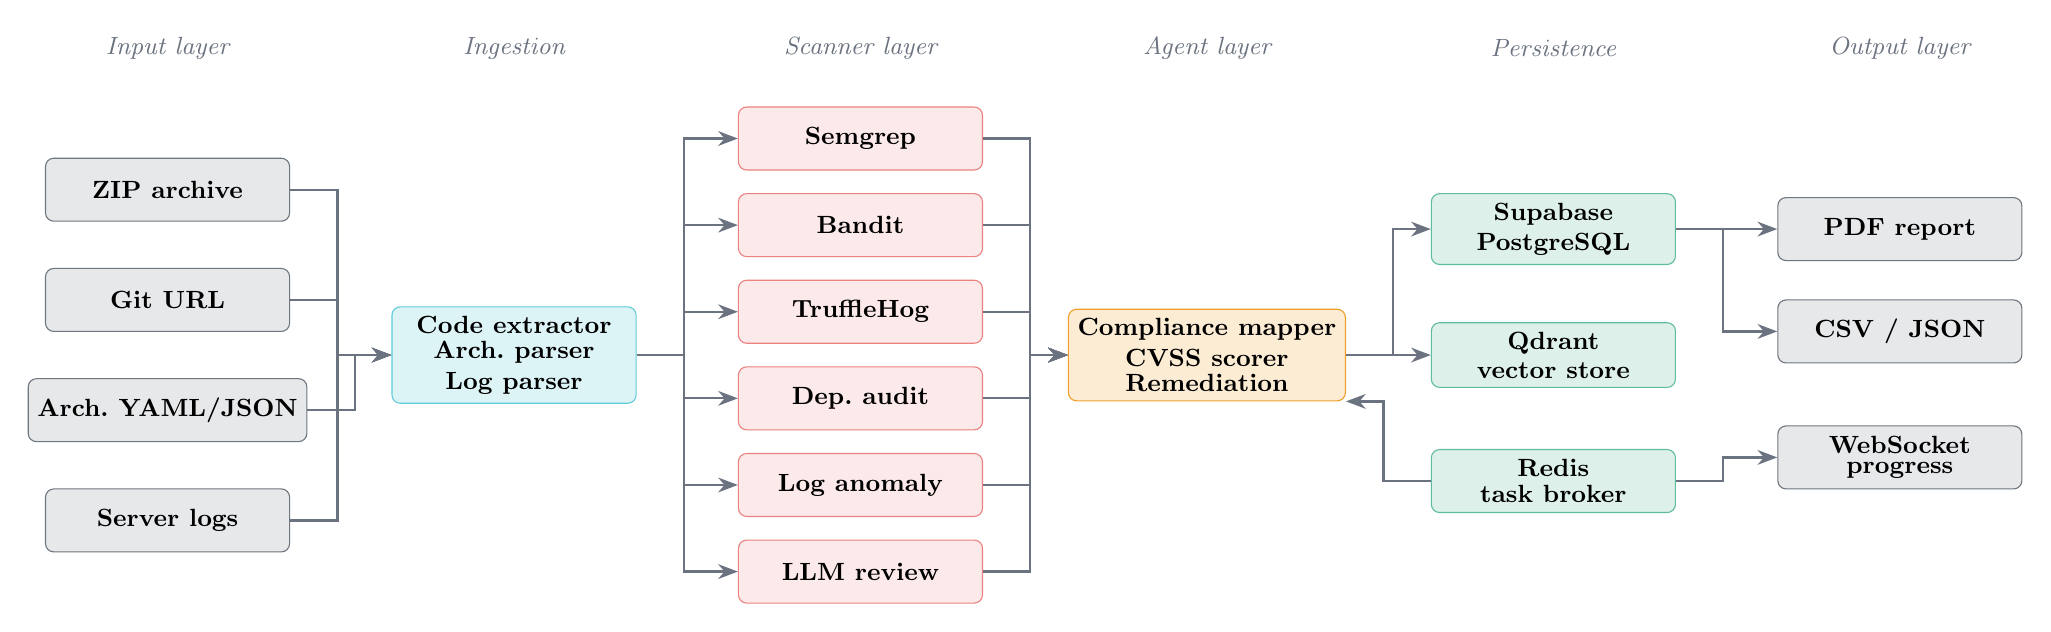
\begin{tikzpicture}[
  box/.style={rectangle, rounded corners=3pt, minimum width=3.1cm,
    minimum height=0.8cm, draw, font=\small\bfseries, align=center},
  nbox/.style={box, fill=TLNavy!10, draw=TLNavy!60},
  cbox/.style={box, fill=TLCyan!15, draw=TLCyan!70},
  rbox/.style={box, fill=TLRed!12,  draw=TLRed!70},
  obox/.style={box, fill=TLOrange!20, draw=TLOrange},
  gbox/.style={box, fill=TLGreen!15, draw=TLGreen!70},
  hdr/.style={font=\small\itshape, text=TLGray},
  arr/.style={-{Stealth[length=2.5mm]}, thick, TLGray}]
% headers
\node[hdr] at (0,3.9)    {Input layer};
\node[hdr] at (4.4,3.9)  {Ingestion};
\node[hdr] at (8.8,3.9)  {Scanner layer};
\node[hdr] at (13.2,3.9) {Agent layer};
\node[hdr] at (17.6,3.9) {Persistence};
\node[hdr] at (22.0,3.9) {Output layer};
% inputs
\node[nbox] (zip)  at (0,2.1)  {ZIP archive};
\node[nbox] (git)  at (0,0.7)  {Git URL};
\node[nbox] (yaml) at (0,-0.7) {Arch.\ YAML/JSON};
\node[nbox] (logs) at (0,-2.1) {Server logs};
% ingestion
\node[cbox] (ing) at (4.4,0) {\shortstack{Code extractor\\Arch.\ parser\\Log parser}};
% scanners
\node[rbox] (sg)  at (8.8,2.75)  {Semgrep};
\node[rbox] (ban) at (8.8,1.65)  {Bandit};
\node[rbox] (tfh) at (8.8,0.55)  {TruffleHog};
\node[rbox] (dep) at (8.8,-0.55) {Dep.\ audit};
\node[rbox] (ano) at (8.8,-1.65) {Log anomaly};
\node[rbox] (llm) at (8.8,-2.75) {LLM review};
% agent
\node[obox] (agt) at (13.2,0) {\shortstack{Compliance mapper\\CVSS scorer\\Remediation}};
% persistence
\node[gbox] (pg)  at (17.6,1.6)  {\shortstack{Supabase\\PostgreSQL}};
\node[gbox] (qdr) at (17.6,0)    {\shortstack{Qdrant\\vector store}};
\node[gbox] (red) at (17.6,-1.6) {\shortstack{Redis\\task broker}};
% output
\node[nbox] (pdf) at (22.0,1.6)  {PDF report};
\node[nbox] (csv) at (22.0,0.3)  {CSV / JSON};
\node[nbox] (ws)  at (22.0,-1.3) {\shortstack{WebSocket\\progress}};
% arrows
\foreach \n in {zip,git,yaml,logs}{\draw[arr] (\n.east) -- ++(0.6,0) |- (ing.west);}
\foreach \n in {sg,ban,tfh,dep,ano,llm}{
  \draw[arr] (ing.east) -- ++(0.6,0) |- (\n.west);
  \draw[arr] (\n.east)  -- ++(0.6,0) |- (agt.west);}
\draw[arr] (agt.east) -- ++(0.6,0) |- (pg.west);
\draw[arr] (agt.east) -- (qdr.west);
\draw[arr] (red.west) -- ++(-0.6,0) |- (agt.south east);
\draw[arr] (pg.east) -- (pdf.west);
\draw[arr] (pg.east) -- ++(0.6,0) |- (csv.west);
\draw[arr] (red.east) -- ++(0.6,0) |- (ws.west);
\end{tikzpicture}}
\caption{ThreatLens high-level architecture. Data flows left to right through
six layers: input, ingestion, multi-scanner analysis, LLM-agent compliance
mapping, persistence, and structured output.}
\label{fig:architecture}
\end{figure*}

\subsection{Technology Stack}
\Cref{tab:stack} summarizes the technology stack. The system combines an
asynchronous FastAPI~\cite{fastapi} application with LangChain~\cite{langchain}
orchestration, Qdrant~\cite{qdrant} similarity search, Celery~\cite{celery}
distributed task queues, Supabase~\cite{supabase} for authenticated persistence
and object storage, and WeasyPrint~\cite{weasyprint} for PDF rendering.

\begin{table*}[!t]
\caption{ThreatLens Technology Stack by Layer}
\label{tab:stack}
\centering\tsz
\renewcommand{\arraystretch}{1.1}
\begin{tabularx}{\textwidth}{@{}lXX@{}}
\toprule
\textbf{Layer} & \textbf{Technology} & \textbf{Rationale}\\
\midrule
API server        & FastAPI 0.110 + Uvicorn (Python 3.11) & Async-first; auto-generated OpenAPI docs\\
LLM inference     & Groq API, Llama 3 70B & Low-latency inference; 8k-token context\\
LLM orchestration & LangChain 0.2 & Structured chain/agent composition\\
Embeddings        & \texttt{all-MiniLM-L6-v2} (384-d) & Strong recall at low compute cost\\
Vector store      & Qdrant (Docker) & Cosine search; metadata filtering\\
Task queue        & Celery 5.x + Redis 7 & Distributed async execution; beat scheduler\\
Authentication    & Supabase Auth + JWKS & Managed OAuth; PKCE flow; RLS\\
Database          & Supabase PostgreSQL 15, SQLAlchemy 2, Alembic & Row-level security; async ORM\\
Storage           & Supabase Storage (private buckets) & Signed URLs; ownership-locked paths\\
PDF               & WeasyPrint 60, Jinja2 3, matplotlib 3.9 & Pure Python; no browser dependency\\
Frontend          & TanStack Start, React 18, TypeScript, Vite 5 & File-based routing; SSR-ready\\
State management  & TanStack Query v5 & Stale-while-revalidate; polling hooks\\
\bottomrule
\end{tabularx}
\end{table*}

\subsection{Repository Layout}
The backend resides in a \texttt{threatlens/} directory alongside a separate
\texttt{src/} TanStack frontend. Backend modules are partitioned into eleven
subdirectories under \texttt{app/}: \texttt{auth/} (JWT verifier and permission
guards), \texttt{models/} (SQLAlchemy ORM models), \texttt{schemas/} (Pydantic~v2
models), \texttt{api/} (FastAPI routes), \texttt{storage/} (Supabase Storage
wrappers), \texttt{ingestion/} (code extractor, architecture and log parsers),
\texttt{scanners/} (the six scanners), \texttt{rag/} (embedder, Qdrant client,
retriever, chunkers), \texttt{agent/} (compliance mapper, CVSS scorer,
remediation planner, summary writer), \texttt{report/} (PDF generator, uploader,
Jinja2 templates), and \texttt{tasks/} (Celery application and tasks).

%====================================================================
\section{RAG Knowledge Base}
\label{sec:rag}
%====================================================================

\subsection{Knowledge Corpus}
The knowledge base encodes 534 control clauses from five frameworks plus two
vulnerability reference catalogs. \Cref{tab:corpus} gives the composition.

\begin{table}[!t]
\caption{RAG Corpus Composition by Framework}
\label{tab:corpus}
\centering\tsz
\begin{tabularx}{\columnwidth}{@{}llXr@{}}
\toprule
\textbf{Framework} & \textbf{Chunk unit} & \textbf{Example IDs} & \textbf{Chunks}\\
\midrule
GDPR          & Article         & Art.5, Art.32, Art.83 & 89\\
SOC 2 Type II & Common criteria & CC6.1--CC9.1          & 67\\
ISO 27001     & Annex A control & A.5.14--A.8.28        & 114\\
PCI DSS v4.0  & Requirement     & Req.2.2.7--Req.11.3.1 & 156\\
NIST CSF 2.0  & Subcategory     & GV.OC-01--RS.MA-01    & 108\\
NVD CVEs      & CVE entry       & CVE-YYYY-NNNNN        & Variable\\
OWASP Top 10  & Category        & A01--A10              & 10\\
\midrule
\multicolumn{3}{@{}l}{\textbf{Total (five compliance frameworks)}} & \textbf{534}\\
\bottomrule
\end{tabularx}
\end{table}

\subsection{Chunking Strategy}
Each framework is chunked at its logical unit of compliance obligation. A GDPR
chunk holds one article with its normative text and guidance; a PCI~DSS chunk
holds one numbered requirement. This granularity keeps retrieved chunks specific
enough to serve as evidence of violation while remaining semantically
discoverable. Each chunk is a dictionary with the structure in \Cref{lst:chunk}
before embedding.

\begin{lstlisting}[language=Python, label={lst:chunk},
  caption={Chunk data structure for the compliance knowledge base.}]
{
    "text": "Art.32 -- Security of processing\n\n"
            "Taking into account the state of the art, "
            "the costs of implementation and the nature, "
            "scope, context and purposes of processing "
            "... the controller and the processor shall "
            "implement appropriate technical and "
            "organisational measures ...",
    "metadata": {
        "framework":       "GDPR",
        "control_id":      "Art.32",
        "control_title":   "Security of processing",
        "category":        "Technical Measures",
        "severity_weight": 0.9,
    }
}
\end{lstlisting}

\subsection{Embedding Model}
ThreatLens uses \texttt{all-MiniLM-L6-v2}, a 22M-parameter sentence transformer
that produces 384-dimensional normalized vectors and follows the Sentence-BERT
architecture~\cite{reimers2019}. The model is loaded once through the singleton
in \Cref{lst:embedder}, avoiding repeated 90\,MB disk reads during scans.

\begin{lstlisting}[language=Python, label={lst:embedder},
  caption={Singleton embedder to avoid repeated model loading.}]
from sentence_transformers import SentenceTransformer

_model: SentenceTransformer | None = None

def get_encoder() -> SentenceTransformer:
    global _model
    if _model is None:
        _model = SentenceTransformer("all-MiniLM-L6-v2")
    return _model

def encode_text(text: str) -> list[float]:
    return get_encoder().encode(text).tolist()
\end{lstlisting}

\subsection{Qdrant Vector Store}
Qdrant~\cite{qdrant} runs as a Docker service on port 6333. The collection uses
cosine distance and 384-dimensional vectors (\Cref{lst:qdrant}). Chunks are
upserted in batches of 100, and the one-time seed script
(\texttt{scripts/seed\_rag.py}) runs all seven chunkers, embedding generation,
and batch upserts in under four minutes on a modern workstation.

\begin{lstlisting}[language=Python, label={lst:qdrant},
  caption={Qdrant collection initialization.}]
from qdrant_client import QdrantClient
from qdrant_client.models import (
    Distance, VectorParams)

def create_collection(client: QdrantClient,
                      name: str) -> None:
    client.recreate_collection(
        collection_name=name,
        vectors_config=VectorParams(
            size=384,
            distance=Distance.COSINE,
        ),
    )
\end{lstlisting}

\subsection{Retrieval Function}
At scan time, the finding text is embedded and searched against the collection,
optionally filtered by framework to improve precision (\Cref{lst:retrieve}).

\begin{lstlisting}[language=Python, label={lst:retrieve},
  caption={Core retrieval function with optional framework filter.}]
from qdrant_client.models import (
    Filter, FieldCondition, MatchAny)

def retrieve_relevant_controls(
    finding_text: str,
    frameworks: list[str] | None = None,
    top_k: int = 10,
) -> list[dict]:
    vector = encode_text(finding_text)
    qfilter = None
    if frameworks:
        qfilter = Filter(must=[
            FieldCondition(
                key="metadata.framework",
                match=MatchAny(any=frameworks),
            )
        ])
    results = get_qdrant().search(
        collection_name=settings.QDRANT_COLLECTION,
        query_vector=vector,
        query_filter=qfilter,
        limit=top_k,
        with_payload=True,
    )
    return [
        {
          "control_id":    r.payload["metadata"]["control_id"],
          "control_title": r.payload["metadata"]["control_title"],
          "framework":     r.payload["metadata"]["framework"],
          "text":          r.payload["text"],
          "score":         r.score,
        }
        for r in results
    ]
\end{lstlisting}

%====================================================================
\section{Scanner Layer}
\label{sec:scanners}
%====================================================================

\subsection{Scanner Architecture}
The scanner layer comprises six modules with a common interface: each accepts a
filesystem path (or parsed data structure), runs its analysis, and returns
\texttt{FindingCreate} objects with normalized severity, CWE identifier, and
file/line provenance. \Cref{fig:scanners} shows the flow from the scanners
through deduplication to storage.

\begin{figure*}[!t]
\centering
\resizebox{\textwidth}{!}{%
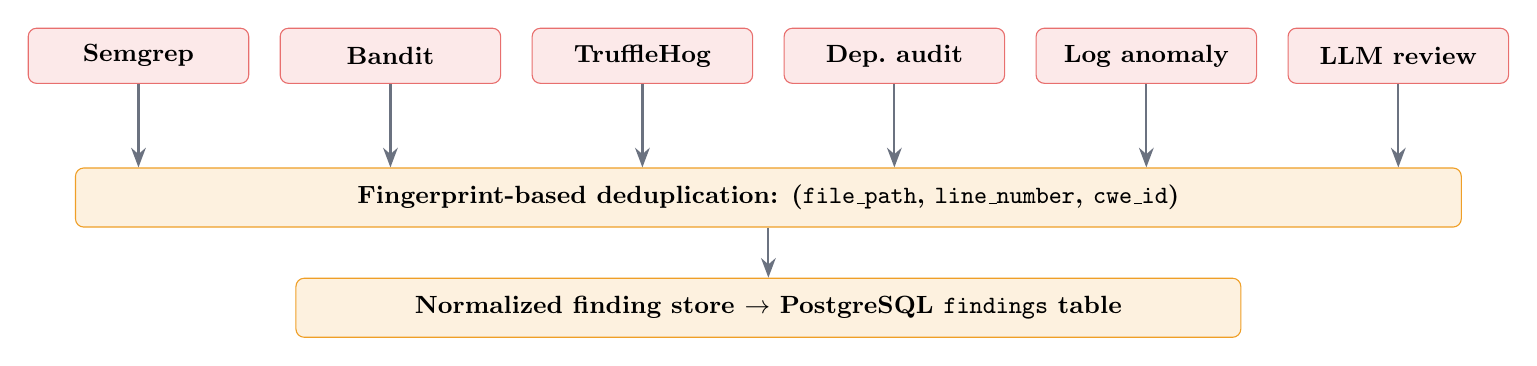
\begin{tikzpicture}[
  sbox/.style={rectangle, rounded corners=3pt, minimum width=2.8cm,
    minimum height=0.7cm, draw=TLRed!80, fill=TLRed!12,
    font=\small\bfseries, align=center},
  mbox/.style={rectangle, rounded corners=3pt, minimum height=0.75cm,
    draw=TLOrange, fill=TLOrange!15, font=\small\bfseries, align=center},
  arr/.style={-{Stealth[length=2.5mm]}, thick, TLGray}]
\node[sbox] (sg)  at (0,0)    {Semgrep};
\node[sbox] (ban) at (3.2,0)  {Bandit};
\node[sbox] (tfh) at (6.4,0)  {TruffleHog};
\node[sbox] (dep) at (9.6,0)  {Dep.\ audit};
\node[sbox] (ano) at (12.8,0) {Log anomaly};
\node[sbox] (llm) at (16.0,0) {LLM review};
\node[mbox, minimum width=17.6cm] (dedup) at (8.0,-1.8)
  {Fingerprint-based deduplication:
   (\texttt{file\_path}, \texttt{line\_number}, \texttt{cwe\_id})};
\node[mbox, minimum width=12cm] (norm) at (8.0,-3.2)
  {Normalized finding store $\rightarrow$ PostgreSQL \texttt{findings} table};
\foreach \n in {sg,ban,tfh,dep,ano,llm}{\draw[arr] (\n.south) -- (\n.south |- dedup.north);}
\draw[arr] (dedup) -- (norm);
\end{tikzpicture}}
\caption{Scanner layer data flow: six analysis engines, deterministic
deduplication, and normalized persistence.}
\label{fig:scanners}
\end{figure*}

\subsection{Semgrep Static Analysis}
Semgrep~\cite{semgrep} runs as a subprocess against the extracted source tree
with eight community rulesets: \texttt{p/owasp-top-ten}, \texttt{p/python},
\texttt{p/javascript}, \texttt{p/secrets}, \texttt{p/supply-chain},
\texttt{p/jwt}, \texttt{p/sql-injection}, and \texttt{p/xss}. Semgrep's
three-tier severity is mapped to ThreatLens's schema as in \Cref{tab:semgrep_sev}.

\begin{table}[!t]
\caption{Semgrep-to-ThreatLens Severity Mapping}
\label{tab:semgrep_sev}
\centering\tsz
\begin{tabular}{@{}ll@{}}
\toprule
\textbf{Semgrep level} & \textbf{ThreatLens severity}\\
\midrule
\texttt{ERROR}   & Critical\\
\texttt{WARNING} & High\\
\texttt{INFO}    & Medium\\
\bottomrule
\end{tabular}
\end{table}

\subsection{Bandit Python AST Analysis}
Bandit~\cite{bandit} analyzes Python abstract syntax trees for patterns such as
\texttt{subprocess.Popen} with \texttt{shell=True}, \texttt{hashlib.md5()}
without \texttt{usedforsecurity=False}, and SQL string concatenation. Severity
is a joint function of Bandit's severity and confidence (\Cref{tab:bandit_sev}).

\begin{table}[!t]
\caption{Bandit Severity and Confidence Mapping}
\label{tab:bandit_sev}
\centering\tsz
\begin{tabular}{@{}lll@{}}
\toprule
\textbf{Bandit severity} & \textbf{Bandit confidence} & \textbf{ThreatLens severity}\\
\midrule
HIGH   & HIGH & Critical\\
HIGH   & any  & High\\
MEDIUM & any  & Medium\\
LOW    & any  & Low\\
\bottomrule
\end{tabular}
\end{table}

\subsection{TruffleHog Secret Detection}
TruffleHog~v3~\cite{trufflehog} detects hardcoded secrets using entropy analysis
and verified pattern matching for over 700 credential types (AWS IAM keys, GitHub
tokens, JWT secrets, private SSH keys, and others). All findings are assigned
Critical severity and CWE-798 (Use of Hard-coded Credentials), consistent with
the CVSS~3.1 base score of 9.8 commonly assigned to exposed credentials.

\subsection{Dependency Vulnerability Audit}
Two sub-runners cover dependency ecosystems. \textbf{pip-audit} scans
\texttt{requirements.txt} and \texttt{Pipfile.lock} against the OSV and NVD
databases. \textbf{npm audit} scans \texttt{package-lock.json} and
\texttt{yarn.lock}, reporting package name, installed version, patched version,
and CVE identifier.

\subsection{Log Anomaly Detection}
The log scanner parses Apache/Nginx access logs, JSON application logs, and
syslog, and applies three rule-based detectors:
\begin{enumerate}[leftmargin=*,nosep,label=\arabic*)]
  \item \textbf{Brute force:} more than 50 failed authentications within any
  five-minute window (High).
  \item \textbf{SQL injection in URLs:} regular-expression matches for
  \texttt{UNION SELECT}, \texttt{--}, \texttt{OR 1=1}, and related patterns
  (Critical).
  \item \textbf{Unusual HTTP methods:} \texttt{TRACE}, \texttt{CONNECT}, and
  \texttt{PROPFIND} (Medium).
\end{enumerate}
In addition, scikit-learn's Isolation Forest is applied to a per-IP feature
matrix of request rate, error rate, and endpoint diversity to flag behavioral
outliers for analyst review.

\subsection{LLM Deep Code Review}
Up to 30 source files per scan (ranked by size and path significance) are sent
to Groq Llama-3-70B for contextual review. Files larger than 8\,KB are truncated
to stay within the 8192-token context window. The system prompt directs the model
to identify authentication and authorization flaws; injection surfaces (SQL,
command, LDAP, XPath); insecure data handling and PII exposure; broken
cryptography; insecure direct object references (IDOR); race conditions
(including time-of-check/time-of-use); and insecure deserialization. The model
must return a JSON array whose objects contain \texttt{title},
\texttt{description}, \texttt{severity}, \texttt{cwe\_id}, \texttt{file\_path},
\texttt{line\_number}, and \texttt{code\_snippet}.

\subsection{Deduplication}
After all scanners finish, findings are deduplicated by the composite key
(\textit{file\_path}, \textit{line\_number}, \textit{cwe\_id}). When several
scanners report the same location and CWE, the finding with the highest severity
is retained. This removes redundant entries and avoids repeated compliance
mapping for identical findings, such as a hardcoded secret reported by both
Semgrep \texttt{p/secrets} and TruffleHog.

%====================================================================
\section{LangChain Agent Chains}
\label{sec:agent}
%====================================================================

\subsection{Chain Architecture}
The agent layer implements four specialized LangChain~\cite{langchain} chains
that convert deduplicated findings into structured compliance intelligence
(\Cref{fig:chains}).

\begin{figure}[!t]
\centering
\resizebox{\columnwidth}{!}{%
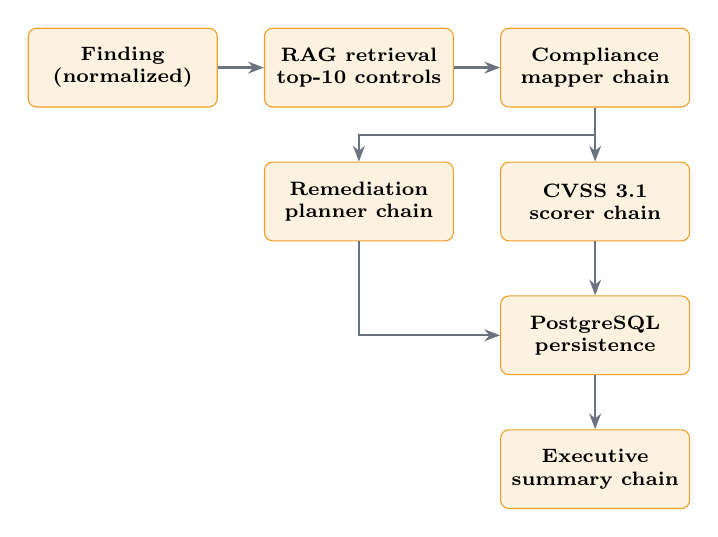
\begin{tikzpicture}[
  cbox/.style={rectangle, rounded corners=3pt, minimum width=2.4cm,
    minimum height=1.0cm, draw=TLOrange, fill=TLOrange!15,
    font=\scriptsize\bfseries, align=center},
  arr/.style={-{Stealth[length=2mm]}, thick, TLGray}]
\node[cbox] (find) at (0,0)    {Finding\\(normalized)};
\node[cbox] (rag)  at (3.0,0)  {RAG retrieval\\top-10 controls};
\node[cbox] (map)  at (6.0,0)  {Compliance\\mapper chain};
\node[cbox] (rem)  at (3.0,-1.7) {Remediation\\planner chain};
\node[cbox] (cvss) at (6.0,-1.7) {CVSS 3.1\\scorer chain};
\node[cbox] (save) at (6.0,-3.4) {PostgreSQL\\persistence};
\node[cbox] (summ) at (6.0,-5.1) {Executive\\summary chain};
\draw[arr] (find) -- (rag);
\draw[arr] (rag) -- (map);
\draw[arr] (map.south) -- (cvss.north);
\draw[arr] (map.south) -- ++(0,-0.35) -| (rem.north);
\draw[arr] (cvss.south) -- (save.north);
\draw[arr] (rem.south) |- (save.west);
\draw[arr] (save.south) -- (summ.north);
\end{tikzpicture}}
\caption{LangChain agent chain sequence for a single finding. RAG retrieval
grounds the compliance mapper with authoritative control text before LLM
invocation.}
\label{fig:chains}
\end{figure}

\subsection{Compliance Mapper}
For each finding, the compliance mapper (i)~embeds the finding description and
retrieves the top-10 most similar control clauses from Qdrant, (ii)~builds a
prompt containing the finding metadata and the full text of the retrieved
clauses, (iii)~invokes Groq Llama-3-70B for a structured JSON object conforming
to the \texttt{ComplianceMappingResult} schema, and (iv)~validates the response
with Pydantic~v2 strict mode, discarding malformed outputs. The output schema is
shown in \Cref{lst:schema}.

\begin{lstlisting}[language=Python, label={lst:schema},
  caption={Pydantic schemas for compliance mapping output.}]
class FrameworkViolation(BaseModel):
    framework: str   # GDPR|SOC2|ISO27001|PCI_DSS|NIST_CSF
    control_id: str  # Art.32 | CC6.1 | A.8.5 | Req.8.3.2
    control_title: str
    violation_description: str
    evidence: str    # specific evidence from the finding

class ComplianceMappingResult(BaseModel):
    violations: list[FrameworkViolation]
    cvss_score: float        # 0.0 - 10.0
    cvss_vector: str         # CVSS:3.1/AV:N/AC:L/...
    remediation_steps: list[str]
    remediation_priority: Literal[
        "immediate",   # < 24 h
        "short-term",  # < 1 week
        "long-term",   # < 1 month
    ]
\end{lstlisting}

\subsection{CVSS 3.1 Auto-Scorer}
The scorer chain evaluates the eight base-metric dimensions (attack vector,
attack complexity, privileges required, user interaction, scope, and
confidentiality, integrity, and availability impact) and returns the base score
and vector string. The LLM derives the score according to the FIRST CVSS~3.1
specification~\cite{CVSS31}, and the result is validated to lie in $[0.0, 10.0]$
before persistence.

\subsection{Remediation Planner}
The planner generates ordered, implementer-focused remediation steps and assigns
an urgency: \textbf{immediate} ($\leq$24\,h) for actively exploitable Critical
findings or those exposing regulated data; \textbf{short-term} ($\leq$1 week) for
High-severity findings that block certification; and \textbf{long-term}
($\leq$1 month) for Medium and Low best-practice gaps.

\subsection{Retry and Rate-Limit Handling}
All Groq API calls use Tenacity exponential backoff (\Cref{lst:retry}). Prompt
injection is mitigated by wrapping all user-supplied code in explicit
\texttt{<code>...</code>} delimiters so that the model does not treat code as
instructions.

\begin{lstlisting}[language=Python, label={lst:retry},
  caption={Tenacity retry decorator for Groq API calls.}]
from tenacity import (retry, stop_after_attempt,
    wait_exponential, retry_if_exception_type)
import httpx

@retry(
    stop=stop_after_attempt(5),
    wait=wait_exponential(multiplier=1, min=2, max=60),
    retry=retry_if_exception_type(httpx.HTTPStatusError),
)
def invoke_groq_with_retry(chain, inputs: dict):
    return chain.invoke(inputs)
\end{lstlisting}

%====================================================================
\section{PDF Report Generator}
\label{sec:report}
%====================================================================

\subsection{Report Architecture}
Reports are produced by a three-stage pipeline: (i)~\textbf{chart generation}, in
which matplotlib renders a color-coded compliance-score bar chart as a
base64-encoded PNG; (ii)~\textbf{HTML rendering}, in which Jinja2 assembles the
report from the templates \texttt{base.html}, \texttt{executive\_summary.html},
\texttt{compliance\_section.html}, and \texttt{findings.html}; and
(iii)~\textbf{PDF conversion}, in which WeasyPrint~\cite{weasyprint} converts the
HTML to PDF while honoring CSS page-break hints.

\subsection{Compliance Score Visualization}
Framework scores use a three-tier scale: \textcolor{TLGreen}{$\blacksquare$}
green for $\geq 80\%$ (compliant or minor gaps),
\textcolor{TLOrange}{$\blacksquare$} orange for 65\%--79\% (partial compliance),
and \textcolor{TLRed}{$\blacksquare$} red for $<65\%$ (non-compliant).

\subsection{Storage and Access Control}
Generated PDFs are uploaded to the \texttt{audit-reports} Supabase Storage bucket
through the Boto3 S3-compatible API. Permanent public URLs are never stored.
Instead, the endpoint \texttt{GET /api/v1/reports/\allowbreak\{id\}/\allowbreak
download} verifies the requester's workspace membership and returns a signed URL
valid for 300\,s, so reports cannot be reached by unauthenticated parties even if
the storage path is known.

\subsection{Export Formats}
In addition to PDF, ThreatLens provides \textbf{CSV export} (all finding fields,
RFC~4180 escaping, and formula-injection mitigation by prefixing cells that begin
with \texttt{=}, \texttt{+}, \texttt{-}, or \texttt{@} with a single quote) and
\textbf{JSON export} (the full machine-readable scan payload, suitable for GRC
platforms or SIEM systems).

%====================================================================
\section{Celery Task Pipeline}
\label{sec:task}
%====================================================================

\subsection{Pipeline Orchestration}
The scan lifecycle is managed by the Celery~\cite{celery} task
\texttt{run\_full\_scan}, which runs nine phases and emits progress updates at
each transition (\Cref{tab:celery}).

\begin{table}[!t]
\caption{Celery Scan Pipeline Phases and Progress Allocation}
\label{tab:celery}
\centering\tsz
\begin{tabularx}{\columnwidth}{@{}rlXr@{}}
\toprule
\textbf{Progress} & \textbf{Phase} & \textbf{Key operations} & \textbf{Retries}\\
\midrule
0--5\%    & Initialization & Create scan record, validate input & 3\\
5--15\%   & Ingestion      & Extract ZIP / clone Git repository & 3\\
15--30\%  & Semgrep        & Static pattern analysis & 1\\
30--40\%  & Bandit         & Python AST analysis & 1\\
40--50\%  & TruffleHog     & Secret and credential scan & 1\\
50--70\%  & LLM review     & Per-file Groq deep review & 3\\
70--75\%  & Deduplication  & Fingerprint dedup, DB persist & 1\\
75--95\%  & Compliance map & RAG $\to$ LLM per finding & 3\\
95--100\% & Finalization   & Framework scores, executive summary & 1\\
\bottomrule
\end{tabularx}
\end{table}

\subsection{Error Isolation}
Per-scanner failures are isolated: if Bandit fails (e.g., on a non-Python
codebase), the task logs the exception and continues with an empty result from
that scanner. The master task fails only if ingestion fails (no source to scan)
or if more than two compliance-mapping retries are exhausted.

\subsection{Celery Beat Scheduler}
A weekly task keeps the NVD chunk set current (\Cref{lst:beat}).

\begin{lstlisting}[language=Python, label={lst:beat},
  caption={Celery Beat schedule for weekly NVD CVE synchronization.}]
from celery.schedules import crontab

celery_app.conf.beat_schedule = {
    "sync-nvd-cves": {
        "task": "app.tasks.scan_task.sync_nvd_cves",
        "schedule": crontab(hour=2, minute=0,
                            day_of_week=0),
    },
}
\end{lstlisting}

%====================================================================
\section{Authentication and Multi-Tenancy}
\label{sec:auth}
%====================================================================

\subsection{Supabase Auth Integration}
Authentication is delegated to Supabase Auth~\cite{supabase}, which manages
signup, e-mail verification, the PKCE OAuth flow, password reset, and token
refresh; FastAPI never receives or stores passwords. \Cref{fig:auth} shows the
JWKS-based JWT verification flow.

\begin{figure}[!t]
\centering
\resizebox{\columnwidth}{!}{%
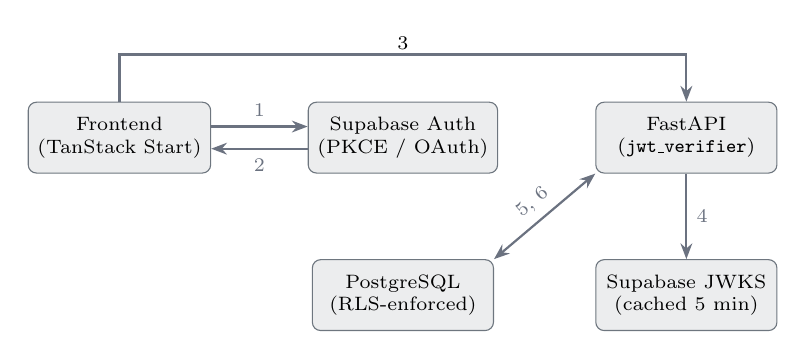
\begin{tikzpicture}[
  abox/.style={rectangle, rounded corners=3pt, minimum width=2.3cm,
    minimum height=0.9cm, draw=TLNavy!60, fill=TLNavy!8,
    font=\scriptsize, align=center},
  arr/.style={-{Stealth[length=2mm]}, thick, TLGray},
  bi/.style={{Stealth[length=2mm]}-{Stealth[length=2mm]}, thick, TLGray}]
\node[abox] (fe)   at (0,0)    {Frontend\\(TanStack Start)};
\node[abox] (supa) at (3.6,0)  {Supabase Auth\\(PKCE / OAuth)};
\node[abox] (api)  at (7.2,0)  {FastAPI\\(\texttt{jwt\_verifier})};
\node[abox] (db)   at (3.6,-2) {PostgreSQL\\(RLS-enforced)};
\node[abox] (jwks) at (7.2,-2) {Supabase JWKS\\(cached 5 min)};
\draw[arr] ([yshift=4pt]fe.east) -- node[above,font=\scriptsize]{1} ([yshift=4pt]supa.west);
\draw[arr] ([yshift=-4pt]supa.west) -- node[below,font=\scriptsize]{2} ([yshift=-4pt]fe.east);
\draw[arr] (fe.north) -- ++(0,0.6) -| (api.north);
\node[font=\scriptsize] at (3.6,1.2) {3};
\draw[arr] (api.south) -- node[right,font=\scriptsize]{4} (jwks.north);
\draw[bi] (api.south west) -- node[above,sloped,font=\scriptsize]{5, 6} (db.north east);
\end{tikzpicture}}
\caption{Authentication flow. (1) The frontend signs in through Supabase Auth;
(2) an access token is returned; (3) the token is sent to FastAPI as a Bearer
credential; (4) FastAPI verifies the signature against cached JWKS; (5)
workspace membership is checked and (6) row-level-security-filtered data is
returned.}
\label{fig:auth}
\end{figure}

\subsection{Workspace Multi-Tenancy}
All application objects (scans, findings, reports, storage artifacts) belong to a
workspace through a \texttt{workspace\_id} foreign key. Row-level security
policies on \texttt{scans}, \texttt{findings}, \texttt{compliance\_violations},
and \texttt{reports} ensure that an authenticated session can only read rows from
workspaces where the user is a member. Membership supports four roles:
\textbf{Owner} (all operations, including workspace deletion), \textbf{Admin}
(create/delete scans, generate reports, manage members), \textbf{Analyst}
(create scans; view all findings and reports), and \textbf{Viewer} (read-only).

\subsection{Rate Limiting}
The \texttt{slowapi} middleware enforces per-user, per-workspace limits derived
from the verified JWT subject: \texttt{POST /api/v1/scans} at 10 requests per
hour, report generation at 5 per hour, and \texttt{GET} endpoints at 100 per
minute. Rate-limited responses carry a \texttt{Retry-After} header.

\subsection{WebSocket Progress Channel}
Progress is delivered over \texttt{WS /api/v1/ws/scans/\allowbreak\{scan\_id\}}.
The client must send an authentication message within five seconds of opening
the connection (\Cref{lst:ws}); the server then sends progress messages every two
seconds while the scan runs. If the WebSocket fails or drops, the frontend falls
back to authenticated 3-second polling with TanStack Query.

\begin{lstlisting}[language=JSONC, label={lst:ws},
  caption={WebSocket authentication and progress messages.}]
# Initial client message (within 5 s)
{
  "type": "authenticate",
  "access_token": "<supabase-access-token>"
}

# Server progress messages (every 2 s while running)
{
  "status": "running",
  "progress": 42,
  "finding_count": 7
}
\end{lstlisting}

%====================================================================
\section{Frontend Integration}
\label{sec:frontend}
%====================================================================

\subsection{Design System}
The frontend uses a neo-brutalist design language with a dark navy/cyan primary
palette and orange/gold accents. Components are divided into
\texttt{components/brutal/} (layout primitives: \texttt{AppShell},
\texttt{BrutalButton}, \texttt{BrutalBadge}, \texttt{ThemeToggle}) and
\texttt{components/ui/} (53 domain components, e.g., \texttt{SeverityBadge},
\texttt{DataTable}, \texttt{CoverageBar}, \texttt{CodePanel},
\texttt{PipelineStep}, \texttt{Progress}).

\subsection{Route-to-Endpoint Mapping}
\Cref{tab:routes} maps each frontend route to the backend endpoints it consumes.

\begin{table*}[!t]
\caption{Frontend Route to Backend Endpoint Mapping}
\label{tab:routes}
\centering\tsz
\begin{tabularx}{\textwidth}{@{}llX@{}}
\toprule
\textbf{Route file} & \textbf{URL path} & \textbf{Backend endpoints}\\
\midrule
\texttt{index.tsx} & \texttt{/} & Static (no API calls)\\
\texttt{dashboard.tsx} & \texttt{/dashboard} & \texttt{GET /api/v1/scans}, \texttt{GET /api/v1/frameworks}\\
\texttt{new-scan.tsx} & \texttt{/new-scan} & \texttt{GET /api/v1/frameworks}, \texttt{POST /api/v1/scans} (then storage upload), \texttt{POST /api/v1/scans/\{id\}/start}\\
\texttt{findings.tsx} & \texttt{/findings} & \texttt{GET /api/v1/scans/\{id\}/findings} (severity and framework filters)\\
\texttt{reports.tsx} & \texttt{/reports} & \texttt{GET /api/v1/reports}, \texttt{POST /api/v1/scans/\{id\}/reports}\\
\texttt{reports.\$id.tsx} & \texttt{/reports/:id} & \texttt{GET /api/v1/reports/\{id\}/download}, \texttt{GET /api/v1/scans/\{id\}/findings}\\
\bottomrule
\end{tabularx}
\end{table*}

\subsection{Mock-to-Live Migration}
The frontend was first built against a \texttt{src/lib/mock-data.ts} module
exporting six data constants. Migration follows progressive replacement: as each
backend part is completed (\Cref{app:timeline_ref}), the corresponding mock
constant is replaced by a TanStack Query hook. A 15-item checklist tracks the
migration, and the last \texttt{mock-data.ts} imports are removed in Part~8.

\subsection{TypeScript Type Contracts}
Backend Pydantic schemas are mirrored as TypeScript interfaces in
\texttt{src/lib/api/types.ts} for compile-time safety across the
frontend--backend boundary (\Cref{lst:ts}).

\begin{lstlisting}[language=TypeScript, label={lst:ts},
  caption={Canonical TypeScript type definitions (excerpt).}]
type Severity = "critical"|"high"|"medium"|"low";
type ScanStatus =
  "pending"|"running"|"completed"|"failed";
type ScanType =
  "codebase"|"architecture"|"logs"|"full";

interface ComplianceViolation {
  framework: string;
  control_id: string;
  control_title: string;
  violation_description: string;
  evidence: string;
}

interface FindingDetail {
  id: string;
  title: string;
  description: string;
  severity: Severity;
  cvss_score: number;
  cvss_vector: string;
  cwe_id: string;
  file_path: string;
  line_number: number | null;
  code_snippet: string | null;
  source: string;
  violations: ComplianceViolation[];
  remediation_steps: string[];
  remediation_priority:
    "immediate"|"short-term"|"long-term";
}
\end{lstlisting}

%====================================================================
\section{Empirical Evaluation}
\label{sec:eval}
%====================================================================

\subsection{Test Environment}
Evaluation ran on a workstation with an Intel Core i7-12700H CPU, an NVIDIA
RTX~4060 GPU (8\,GB), 32\,GB DDR5 RAM, and a 1\,TB NVMe SSD. The backend ran in
Docker with PostgreSQL~15, Redis~7, and Qdrant alongside the FastAPI application
and four Celery workers. A deliberately vulnerable Flask application
(\texttt{tests/fixtures/vulnerable\_app.py}) was the primary target.

\subsection{Scanner Results}
\Cref{tab:scanner_results} summarizes detection results on the fixture, which
was crafted to contain representative instances of each vulnerability class.

\begin{table}[!t]
\caption{Scanner Detection Results on the Vulnerable Flask Fixture}
\label{tab:scanner_results}
\centering\tsz
\begin{tabularx}{\columnwidth}{@{}lXccc@{}}
\toprule
\textbf{Scanner} & \textbf{Target} & \textbf{Exp.} & \textbf{Det.} & \textbf{FP}\\
\midrule
Semgrep     & SQLi, XSS, JWT misuse & 12 & 11 & 2\\
Bandit      & Hardcoded password, \texttt{eval()}, MD5 & 8 & 8 & 1\\
TruffleHog  & AWS key, GitHub token, JWT secret & 3 & 3 & 0\\
Dep.\ audit & 3 CVE-listed packages & 3 & 3 & 0\\
Log anomaly & Brute force, SQLi in URL & 5 & 4 & 1\\
LLM review  & IDOR, race condition, broken auth & 6 & 5 & 2\\
\midrule
\textbf{Total} & & \textbf{37} & \textbf{34} & \textbf{6}\\
\bottomrule
\end{tabularx}
\par\smallskip\raggedright\scriptsize Exp.: expected; Det.: detected; FP: false positives.
\end{table}

The aggregate detection rate was $34/37 = 91.9\%$. TruffleHog and the dependency
auditor achieved perfect recall and zero false positives on their vulnerability
classes.

\subsection{RAG Retrieval Precision}
Retrieval precision was evaluated on a held-out set of 50 (finding text,
expected control set) pairs, with expected sets annotated manually by a
compliance professional. \Cref{tab:rag_eval} reports precision of the top-$k$
retrieved controls per framework.

\begin{table}[!t]
\caption{RAG Retrieval Precision by Framework}
\label{tab:rag_eval}
\centering\tsz
\begin{tabular}{@{}lccc@{}}
\toprule
\textbf{Framework} & \textbf{P@5} & \textbf{P@10} & \textbf{Rank of 1st relevant}\\
\midrule
GDPR         & 0.91 & 0.88 & 1.4\\
SOC 2        & 0.89 & 0.86 & 1.6\\
ISO 27001    & 0.93 & 0.89 & 1.2\\
PCI DSS v4.0 & 0.88 & 0.84 & 1.7\\
NIST CSF 2.0 & 0.90 & 0.87 & 1.5\\
\midrule
\textbf{Mean} & \textbf{0.902} & \textbf{0.868} & \textbf{1.48}\\
\bottomrule
\end{tabular}
\end{table}

A mean P@10 of 0.868 indicates that \texttt{all-MiniLM-L6-v2} is sufficiently
discriminative across the control vocabularies of the five frameworks. The mean
rank of 1.48 for the first relevant control means that a relevant control
typically appears in the top two results.

\subsection{End-to-End Pipeline Performance}
\Cref{tab:perf} reports wall-clock time per phase on the test codebase (47
source files, 8,400 lines of code).

\begin{table}[!t]
\caption{Pipeline Phase Timing (47-File Codebase, Four Celery Workers)}
\label{tab:perf}
\centering\tsz
\begin{tabular}{@{}lrr@{}}
\toprule
\textbf{Phase} & \textbf{Time (s)} & \textbf{Share (\%)}\\
\midrule
Ingestion (ZIP extract)            &  1.2 &  1.5\\
Semgrep                            & 14.3 & 17.7\\
Bandit                             &  3.1 &  3.8\\
TruffleHog                         &  8.7 & 10.8\\
Dependency audit                   &  6.2 &  7.7\\
LLM review (30 files, Groq)        & 28.4 & 35.2\\
Deduplication                      &  0.3 &  0.4\\
Compliance mapping (34 findings)   & 17.6 & 21.8\\
Report generation                  &  0.9 &  1.1\\
\midrule
\textbf{Total}                     & \textbf{80.7} & \textbf{100.0}\\
\bottomrule
\end{tabular}
\end{table}

LLM inference accounts for 57.0\% of total time (35.2\% deep review plus 21.8\%
compliance mapping), so Groq latency is the dominant bottleneck. Running the
scanner phases as a Celery group chord shortens the critical path, but the LLM
phases remain sequential because of Groq rate limits.

\subsection{Test Suite Results}
The default test suite (excluding opt-in smoke tests) yields 89 passing and 4
skipped tests across unit tests for all eight implementation parts. The four
skipped tests are smoke tests that require either installed scanner binaries or
a valid Groq API key, and they run separately (\Cref{lst:smoke}).

\begin{lstlisting}[language=bash, label={lst:smoke},
  caption={Smoke tests requiring external tools or credentials.}]
# Real scanner smoke tests (tools installed)
THREATLENS_RUN_SCANNER_SMOKE=1 \
  pytest tests/test_part4_smoke.py

# Groq LLM smoke test (needs GROQ_API_KEY)
THREATLENS_RUN_GROQ_SMOKE=1 \
  pytest tests/test_part4_smoke.py
\end{lstlisting}

%====================================================================
\section{Security Design}
\label{sec:security}
%====================================================================

\subsection{Threat Model}
ThreatLens handles sensitive artifacts (proprietary source code, security
findings, and compliance violation records) on behalf of tenants. The primary
threats are (i)~\textbf{cross-tenant data leakage}, (ii)~\textbf{prompt
injection} through malicious code in uploaded codebases, (iii)~\textbf{ZIP bomb
and path traversal} attacks on extraction, (iv)~\textbf{scanner abuse} to
execute arbitrary code on the server, and (v)~\textbf{credential exfiltration}
of Groq, Supabase, or database credentials through the scanner subprocess
environment. \Cref{tab:security} lists the mitigations.

\subsection{Mitigations}
\begin{table*}[!t]
\caption{Security Mitigations by Threat Category}
\label{tab:security}
\centering\tsz
\begin{tabularx}{\textwidth}{@{}lX@{}}
\toprule
\textbf{Threat} & \textbf{Mitigation}\\
\midrule
Cross-tenant leakage    & Supabase RLS on all application tables; \texttt{workspace\_id} in every query; signed report URLs scoped to the authenticated requester.\\
Prompt injection        & Finding text wrapped in explicit XML-style delimiters; model instructed to treat delimited content as opaque.\\
ZIP bomb                & Compressed/extracted size ratio check (maximum 100$\times$); maximum of 1000 extracted files.\\
Path traversal          & All extracted paths sanitized; patterns containing \texttt{../} rejected.\\
Scanner code execution  & No uploaded code is executed; all scanners are static. Subprocess environments are stripped of credentials.\\
Subprocess timeouts     & 300-second timeout on all scanner subprocesses.\\
LLM hallucination       & Pydantic strict-mode validation of all LLM outputs; malformed responses discarded.\\
CSV formula injection   & Cell values prefixed with a single quote if they begin with \texttt{=}, \texttt{+}, \texttt{-}, or \texttt{@}.\\
Token leakage           & WebSocket access tokens never placed in URL query strings; authentication via initial message only.\\
\bottomrule
\end{tabularx}
\end{table*}

\subsection{Operational Security}
Docker containers run as non-root users on the minimal
\texttt{python:3.11-slim} base image. The \texttt{.env} file is excluded from
version control, and \texttt{.env.example} supplies placeholders. The
\texttt{SECRET\_KEY} is at least 64 characters of cryptographically random data.
Celery uses the JSON serializer (not pickle) to prevent deserialization attacks,
and \texttt{result\_expires=3600} prevents indefinite accumulation of sensitive
task results in Redis. Supabase Storage bucket policies restrict object access
to the owning workspace.

%====================================================================
\section{Conclusion}
\label{sec:conclusion}
%====================================================================

\subsection{Summary}
ThreatLens shows that combining multi-tool static analysis, LLM-agentic
reasoning, and retrieval-augmented compliance mapping substantially reduces the
manual effort needed to produce an audit-ready security and compliance
assessment. On the test application it achieved a 91.9\% aggregate detection
rate, a mean RAG retrieval precision of 0.868 across five frameworks, and an
end-to-end run time of about 81\,s for a 47-file codebase. The modular design
(eight backend parts, \Cref{app:timeline_ref}) connected through a Celery
pipeline supports incremental deployment and testing, and strict workspace-level
isolation keeps potentially sensitive scan data separated between tenants.

\subsection{Limitations}
\begin{itemize}[leftmargin=*,nosep]
  \item \textbf{LLM latency.} Groq inference accounts for 57\% of pipeline time
  and limits throughput to roughly 45 scans per hour within the current rate
  limits.
  \item \textbf{False positives.} The evaluation produced six false positives
  alongside 34 true detections (precision $\approx 0.85$), which would add noise
  in high-volume environments. Per-scanner confidence thresholds could reduce it.
  \item \textbf{Evaluation scope.} Detection was measured on a single
  self-constructed fixture, so the figures do not generalize to real codebases.
  \item \textbf{Framework currency.} The corpus must be re-seeded when
  frameworks change. NIST CSF~2.0 replaced 1.1 in February 2024, and PCI~DSS
  v4.0.1, a limited revision of v4.0 with no new or removed requirements, was
  published in June 2024 and is now the sole active version.
  \item \textbf{Binary analysis.} Compiled binaries, Docker image layers, and
  infrastructure-as-code (e.g., Terraform state) are not supported.
\end{itemize}

\subsection{Future Work}
Planned work includes (i)~continuous scanning through CI/CD webhooks (GitHub
Actions, GitLab CI); (ii)~dataflow analysis with tools such as CodeQL to detect
second-order injection; (iii)~adding HIPAA, SOX, FedRAMP, and India's Digital
Personal Data Protection Act 2023 to the knowledge base; (iv)~fine-tuning a
compact (e.g., 7B-parameter) compliance LLM to replace general-purpose Llama~3
for mapping; (v)~generating Git diffs or pull requests that apply suggested
fixes; and (vi)~exporting violations to Drata, Vanta, or Secureframe through
their APIs.

%====================================================================
% APPENDICES
%====================================================================
\appendices

\section{Complete API Reference}
\label{app:api}
\Cref{tab:fullapi} lists all REST endpoints and the WebSocket channel.

\begin{table*}[!t]
\caption{Complete ThreatLens REST and WebSocket API Surface}
\label{tab:fullapi}
\centering\tsz
\renewcommand{\arraystretch}{1.05}
\begin{tabularx}{\textwidth}{@{}lllX@{}}
\toprule
\textbf{Method} & \textbf{Path} & \textbf{Auth} & \textbf{Description}\\
\midrule
GET    & \texttt{/health} & None & Service health check\\
GET    & \texttt{/api/v1/auth/me} & JWT & Current user profile and workspace memberships\\
POST   & \texttt{/api/v1/auth/bootstrap} & JWT & Idempotent profile and workspace initialization\\
PATCH  & \texttt{/api/v1/auth/profile} & JWT & Update display name and avatar\\
GET    & \texttt{/api/v1/frameworks} & JWT & List compliance frameworks with chunk counts\\
POST   & \texttt{/api/v1/scans} & JWT & Create scan record and return upload URL\\
POST   & \texttt{/api/v1/scans/\{id\}/start} & JWT & Enqueue scan after upload verification\\
GET    & \texttt{/api/v1/scans} & JWT & List scans for the authenticated workspace\\
GET    & \texttt{/api/v1/scans/\{id\}} & JWT & Scan status, progress, and finding count\\
DELETE & \texttt{/api/v1/scans/\{id\}} & JWT & Delete scan and associated findings\\
GET    & \texttt{/api/v1/scans/\{id\}/findings} & JWT & Paginated findings with severity/framework filter\\
POST   & \texttt{/api/v1/scans/\{id\}/reports} & JWT & Trigger asynchronous PDF report generation\\
GET    & \texttt{/api/v1/reports} & JWT & List reports for the workspace\\
GET    & \texttt{/api/v1/reports/\{id\}/download} & JWT & Short-lived signed download URL (300\,s)\\
GET    & \texttt{/api/v1/scans/\{id\}/export/csv} & JWT & Download findings as RFC 4180 CSV\\
GET    & \texttt{/api/v1/scans/\{id\}/export/json} & JWT & Download findings as JSON\\
WS     & \texttt{/api/v1/ws/scans/\{id\}} & Message & Authenticated scan progress channel\\
\bottomrule
\end{tabularx}
\end{table*}

\section{Environment Variable Reference}
\label{app:env}
\Cref{tab:envvars} lists the backend configuration variables.

\begin{table*}[!t]
\caption{Backend Environment Variables (\texttt{.env})}
\label{tab:envvars}
\centering\tsz
\renewcommand{\arraystretch}{1.05}
\begin{tabularx}{\textwidth}{@{}lXl@{}}
\toprule
\textbf{Variable} & \textbf{Description} & \textbf{Required}\\
\midrule
\texttt{DATABASE\_URL}             & Async SQLAlchemy connection string & Yes\\
\texttt{MIGRATION\_DATABASE\_URL}  & Sync Alembic migration connection string & Yes\\
\texttt{REDIS\_URL}                & Redis broker and result backend URL & Yes\\
\texttt{QDRANT\_HOST}              & Qdrant server hostname & Yes\\
\texttt{QDRANT\_PORT}              & Qdrant server port (default 6333) & No\\
\texttt{QDRANT\_COLLECTION}        & Qdrant collection name & No\\
\texttt{GROQ\_API\_KEY}            & Groq API authentication key & Yes\\
\texttt{SUPABASE\_URL}             & Supabase project URL & Yes\\
\texttt{SUPABASE\_JWKS\_URL}       & JWKS endpoint for JWT verification & Yes\\
\texttt{SUPABASE\_JWT\_ISSUER}     & Expected JWT issuer claim & Yes\\
\texttt{SUPABASE\_JWT\_AUDIENCE}   & Expected JWT audience claim & Yes\\
\texttt{SUPABASE\_SERVICE\_ROLE\_KEY} & Server-only Supabase service key & Yes\\
\texttt{SUPABASE\_SCAN\_BUCKET}    & Private scan-input storage bucket & Yes\\
\texttt{SUPABASE\_REPORT\_BUCKET}  & Private report storage bucket & Yes\\
\texttt{SIGNED\_URL\_TTL\_SECONDS} & Report download URL TTL (default 300) & No\\
\texttt{SECRET\_KEY}               & 64+ character random key (CSRF/sessions) & Yes\\
\texttt{CORS\_ORIGINS}             & Allowed frontend origins (JSON list) & Yes\\
\texttt{DEBUG}                     & Debug mode (False in production) & No\\
\texttt{MAX\_FILE\_SIZE\_MB}       & Maximum upload size in MB & No\\
\bottomrule
\end{tabularx}
\end{table*}

\section{Database Schema Summary}
\label{app:schema}
\Cref{tab:schema} summarizes the ten core PostgreSQL tables; tenancy isolation is
enforced through row-level security.

\begin{table}[!t]
\caption{PostgreSQL Table Inventory}
\label{tab:schema}
\centering\tsz
\begin{tabularx}{\columnwidth}{@{}lllX@{}}
\toprule
\textbf{Table} & \textbf{PK} & \textbf{RLS} & \textbf{Key foreign keys}\\
\midrule
\texttt{auth.users}            & UUID & Managed & --\\
\texttt{profiles}              & UUID & Yes & \texttt{auth.users.id}\\
\texttt{workspaces}            & UUID & Yes & \texttt{profiles.id} (owner)\\
\texttt{workspace\_members}    & UUID & Yes & \texttt{workspaces.id}, \texttt{profiles.id}\\
\texttt{scans}                 & UUID & Yes & \texttt{workspaces.id}\\
\texttt{scan\_artifacts}       & UUID & Yes & \texttt{scans.id}\\
\texttt{findings}              & UUID & Yes & \texttt{scans.id}\\
\texttt{compliance\_violations} & UUID & Yes & \texttt{findings.id}\\
\texttt{reports}               & UUID & Yes & \texttt{scans.id}\\
\texttt{audit\_events}         & UUID & Yes & \texttt{workspaces.id}, \texttt{profiles.id}\\
\bottomrule
\end{tabularx}
\end{table}

\section{Implementation Timeline}
\label{app:timeline_ref}
The eight-part engineering effort followed the schedule in \Cref{tab:timeline}.

\begin{table*}[!t]
\caption{Eight-Part Implementation Timeline with Estimated Effort}
\label{tab:timeline}
\centering\tsz
\begin{tabularx}{\textwidth}{@{}rlXr@{}}
\toprule
\textbf{Part} & \textbf{Weeks} & \textbf{Deliverables} & \textbf{Effort (days)}\\
\midrule
1 & 1    & Foundation: FastAPI, Supabase DB, Redis, Qdrant, Celery, health endpoint & 2--4\\
2 & 2--3 & RAG knowledge base: chunkers, embedder, Qdrant seeding, retriever & 3--5\\
3 & 4--5 & Ingestion layer: ZIP extractor, Git cloner, architecture and log parsers & 3--5\\
4 & 4--7 & Six scanners, deduplication, findings API & 3--5\\
5 & 8    & LangChain chains: compliance mapper, CVSS scorer, remediation planner & 3--5\\
6 & 9    & PDF generator, Jinja2 templates, Supabase Storage, export endpoints & 3--4\\
7 & 6--8 & Celery full pipeline: orchestration, progress, retries, CVE sync & 3--4\\
8 & 10   & Supabase Auth hardening, WebSocket, rate limiting, mock-to-live migration & 3--5\\
\midrule
\multicolumn{3}{@{}l}{\textbf{Total}} & \textbf{23--37}\\
\bottomrule
\end{tabularx}
\end{table*}

%====================================================================
\section*{Acknowledgment}
%====================================================================
The authors thank the project guide and the faculty of the Department of
Computer Science and Engineering, G.~H. Raisoni College of Engineering, Nagpur,
for their guidance. Thanks are also due to the open-source communities behind
Semgrep, Bandit, TruffleHog, LangChain, Qdrant, FastAPI, Supabase, and
WeasyPrint, and to the IEEE GHRCE and Google Developer Groups On Campus GHRCE
student chapters for research and development support.

%====================================================================
% REFERENCES  (numbered in order of first citation, per IEEE style)
%====================================================================
\begin{thebibliography}{00}

\bibitem{GDPR2016}
European Parliament and Council of the European Union, ``Regulation (EU)
2016/679 on the protection of natural persons with regard to the processing of
personal data and on the free movement of such data (General Data Protection
Regulation),'' \textit{Off. J. Eur. Union}, vol.~L119, pp.~1--88, May 2016.

\bibitem{PCIDSS4}
PCI Security Standards Council, ``Payment Card Industry Data Security Standard:
Requirements and testing procedures, v4.0,'' Wakefield, MA, USA, Mar. 2022.

\bibitem{SOC2}
American Institute of Certified Public Accountants, ``2017 Trust services
criteria for security, availability, processing integrity, confidentiality, and
privacy (with revised points of focus---2022),'' AICPA, New York, NY, USA, 2022.

\bibitem{ISO27001}
\textit{Information Security, Cybersecurity and Privacy Protection---Information
Security Management Systems---Requirements}, ISO/IEC Standard 27001:2022, Oct.
2022.

\bibitem{NISTCSF2}
National Institute of Standards and Technology, ``The NIST cybersecurity
framework (CSF) 2.0,'' NIST, Gaithersburg, MD, USA, Cybersecurity White Paper
(CSWP) 29, Feb. 2024, doi: 10.6028/NIST.CSWP.29.

\bibitem{CVSS31}
FIRST.Org, Inc., ``Common Vulnerability Scoring System v3.1: Specification
document,'' Jun. 2019. [Online]. Available:
\url{https://www.first.org/cvss/v3-1/specification-document}

\bibitem{zhou2024llmvuln}
X.~Zhou \textit{et al.}, ``Large language model for vulnerability detection and
repair: Literature review and the road ahead,'' \textit{ACM Trans. Softw. Eng.
Methodol.}, 2024, arXiv:2404.02525.

\bibitem{steenhoek2024finetune}
A.~Steenhoek \textit{et al.}, ``Finetuning large language models for
vulnerability detection,'' \textit{IEEE Access}, 2024, arXiv:2401.17010.

\bibitem{fan2025dlvuln}
G.~Fan \textit{et al.}, ``Deep learning aided software vulnerability detection:
A survey,'' arXiv:2503.04002, 2025.

\bibitem{pnnl2024cyrag}
Pacific Northwest National Laboratory, ``Retrieval augmented generation for
robust cyber defense (CyRAG),'' PNNL, Richland, WA, USA, Tech. Rep.,
arXiv:2402.14160, 2024.

\bibitem{mauri2022stride}
L.~Mauri and E.~Damiani, ``Modeling threats to AI-ML systems using STRIDE,''
\textit{Sensors}, vol.~22, no.~17, Art.~no.~6662, 2022,
doi: 10.3390/s22176662.

\bibitem{setu2023secretbench}
S.~K. Basak, L.~Neil, B.~Reaves, and L.~Williams, ``SecretBench: A dataset of
software secrets,'' in \textit{Proc. 20th IEEE/ACM Int. Conf. Mining Softw.
Repositories (MSR)}, 2023, arXiv:2303.06729.

\bibitem{ma2024seagull}
S.~Ma \textit{et al.}, ``A credential usage study: Flow-aware leakage detection
in open-source projects,'' \textit{IEEE Trans. Inf. Forensics Security}, 2024,
arXiv:2403.00336.

\bibitem{marandi2023devsecops}
M.~Marandi \textit{et al.}, ``Implementing and automating security scanning to a
DevSecOps CI/CD pipeline,'' in \textit{Proc. IEEE World Conf. Commun. Comput.
(WCONF)}, 2023, pp.~1--6, doi: 10.1109/WCONF57249.2023.10370425.

\bibitem{chua2024iforest}
W.~Chua \textit{et al.}, ``Web traffic anomaly detection using Isolation
Forest,'' \textit{Informatics}, vol.~11, no.~4, p.~83, 2024,
doi: 10.3390/informatics11040083.

\bibitem{wang2024vulndeps}
J.~Wang \textit{et al.}, ``A comprehensive study on the impact of vulnerable
dependencies on open-source software,'' in \textit{Proc. IEEE 35th Int. Symp.
Softw. Rel. Eng. (ISSRE)}, 2024, arXiv:2408.08472.

\bibitem{thakur2023}
A.~Thakur, A.~Ganesan, and R.~Srihari, ``Enhancing software vulnerability
detection using large language models,'' arXiv:2401.12169, 2024.

\bibitem{pearce2022asleep}
H.~Pearce, B.~Ahmad, B.~Tan, B.~Dolan-Gavitt, and R.~Karri, ``Asleep at the
keyboard? Assessing the security of GitHub Copilot's code contributions,'' in
\textit{Proc. IEEE Symp. Secur. Privacy (SP)}, 2022, pp.~754--768.

\bibitem{lewis2020rag}
P.~Lewis \textit{et al.}, ``Retrieval-augmented generation for
knowledge-intensive NLP tasks,'' in \textit{Proc. Adv. Neural Inf. Process. Syst.
(NeurIPS)}, vol.~33, 2020, pp.~9459--9474.

\bibitem{veeraReddy2024}
S.~Veera Reddy and D.~Bhattacharyya, ``Hallucination reduction in compliance
LLMs via retrieval-augmented generation,'' \textit{Int. J. Intell. Syst. Appl.},
vol.~16, no.~3, pp.~45--59, 2024.

\bibitem{meli2019}
M.~Meli, M.~R. McNiece, and B.~Reaves, ``How bad can it git? Characterizing
secret leakage in public GitHub repositories,'' in \textit{Proc. Netw. Distrib.
Syst. Secur. Symp. (NDSS)}, San Diego, CA, USA, 2019.

\bibitem{fastapi}
S.~Ram{\'\i}rez. ``FastAPI: Modern, fast web framework for building APIs with
Python.'' [Online]. Available: \url{https://fastapi.tiangolo.com} (accessed
Sep. 30, 2026).

\bibitem{langchain}
H.~Chase. ``LangChain: Building applications with LLMs through composability.''
GitHub. [Online]. Available: \url{https://github.com/langchain-ai/langchain}
(accessed Sep. 30, 2026).

\bibitem{qdrant}
Qdrant Solutions GmbH. ``Qdrant: Vector similarity search engine.'' [Online].
Available: \url{https://qdrant.tech} (accessed Sep. 30, 2026).

\bibitem{celery}
A.~Solem and contributors. ``Celery: Distributed task queue.'' [Online].
Available: \url{https://docs.celeryq.dev} (accessed Sep. 30, 2026).

\bibitem{supabase}
Supabase Inc. ``Supabase: The open-source Firebase alternative.'' [Online].
Available: \url{https://supabase.com} (accessed Sep. 30, 2026).

\bibitem{weasyprint}
Kozea SAS. ``WeasyPrint: The awesome document factory.'' [Online]. Available:
\url{https://weasyprint.org} (accessed Sep. 30, 2026).

\bibitem{reimers2019}
N.~Reimers and I.~Gurevych, ``Sentence-BERT: Sentence embeddings using Siamese
BERT-networks,'' in \textit{Proc. Conf. Empirical Methods Natural Lang. Process.
9th Int. Joint Conf. Natural Lang. Process. (EMNLP-IJCNLP)}, Hong Kong, China,
2019, pp.~3982--3992.

\bibitem{semgrep}
Semgrep, Inc. ``Semgrep: Static analysis at ludicrous speed.'' [Online].
Available: \url{https://semgrep.dev} (accessed Sep. 30, 2026).

\bibitem{bandit}
PyCQA Bandit Contributors. ``Bandit: A security linter for Python.'' [Online].
Available: \url{https://bandit.readthedocs.io} (accessed Sep. 30, 2026).

\bibitem{trufflehog}
Truffle Security Co. ``TruffleHog v3: Secret scanner with verified detectors.''
GitHub. [Online]. Available: \url{https://github.com/trufflesecurity/trufflehog}
(accessed Sep. 30, 2026).

\end{thebibliography}

\end{document}
